\documentclass[11pt,a4paper,oneside]{article}
\usepackage[utf8]{inputenc}
\usepackage[T1]{fontenc}
\usepackage{lmodern}
\usepackage{graphicx}
\graphicspath{ {./resources/images/} }
\usepackage[french]{babel}
\pagestyle{headings}
\author{Bruno Parmentier \and Olivier Marcotte}
\title{Gestion et administration des réseaux - Linux \\[1cm] \emph{Configuration
du réseau avec adressage statique}}
\date{13 mars 2014}
\begin{document}

\begin{titlepage}
\maketitle
\thispagestyle{empty}
\end{titlepage}

\section{Objectif}
Configuration du réseau avec adressage statique.

Dans le local, chaque table possède un numéro. Ce numéro détermine les adresses
du réseau à configurer (4 dans notre cas). La première machine, le routeur et
passerelle de notre réseau (appelons-la \emph{darkstar}), aura l'adresse
\verb#172.16.0.204# (sur eth0). Celle-ci aura accès à internet via
\emph{Iznogoud}, à l'adresse \verb#172.16.0.3#. Cette dernière aura également le
rôle de serveur DNS.

Sur notre réseau, nous créerons deux sous-réseaux : une DMZ (\verb#172.16.14.0#)
et un ``local'' (\verb#172.16.24.0#). La DMZ contiendra une machine
(\emph{dmz-server}) ayant pour adresse \verb#172.16.14.2# et comme passerelle
\verb#172.16.14.1# (eth1 sur \emph{darkstar}) et le local contiendra deux machines
(\emph{local1} et \emph{local2}) ayant respectivement pour adresses
\verb#172.16.24.2# et \verb#172.16.24.3# et comme passerelle \verb#172.16.24.1#
(eth2 sur \emph{darkstar}).

\begin{figure}[htb]
    \begin{center}
        \includegraphics[width=\textwidth]{topologie_reseau.pdf}
        \caption{Topologie du réseau}
        \label{fig:topologie_reseau}
    \end{center}
\end{figure}

\section{Mode opératoire}

\subsection{Configuration de la passerelle}
Modifier le fichier \verb#/etc/rc.d/rc.inet1.conf# sur \emph{darkstar} comme
suit~:
\begin{verbatim}
# Config information for eth0:
IPADDR[0]="172.16.0.204"
NETMASK[0]="255.255.255.0"
USE_DHCP[0]=""
DHCP_HOSTNAME[0]=""

# Config information for eth1:
IPADDR[1]="172.16.14.1"
NETMASK[2]="255.255.255.0"
USE_DHCP[1]=""
DHCP_HOSTNAME[1]=""

# Config information for eth2:
IPADDR[2]="172.16.24.1"
NETMASK[2]="255.255.255.0"
USE_DHCP[2]=""
DHCP_HOSTNAME[2]=""

# Default gateway IP address:
GATEWAY="172.16.0.3"
\end{verbatim}

Pour appliquer les changements sans redémarrer la machine, nous utilisons la
commande \verb#/etc/rc.d/rc.inet1 restart#.

Comme la passerelle fait office de routeur, il faut activer l'IP forwarding.
Pour cela, remplacer 0 par 1 dans le fichier
\verb#/proc/sys/net/ipv4/ip-forward# (version immédiate mais temporaire) ou
rendre exécutable le fichier \verb#/etc/rc.d/rc.ipforward# (version
définitive).

Pour avoir la résolution des noms de domaines, ajouter la ligne suivante dans le
fichier \verb#/etc/resolv.conf#~:
\begin{verbatim}
nameserver      172.16.0.3
\end{verbatim}

\subsection{Configuration des clients}

Comme pour la passerelle, et pour chaque machine du réseau, ajouter la ligne
suivante dans le fichier \verb#/etc/resolv.conf#~:
\begin{verbatim}
nameserver      172.16.0.3
\end{verbatim}


\subsubsection{DMZ}
Modifier le fichier \verb#/etc/rc.d/rc.inet1.conf# sur \emph{dmz-server} comme
suit~:
\begin{verbatim}
# Config information for eth0:
IPADDR[0]="172.16.14.2"
NETMASK[0]="255.255.255.0"
USE_DHCP[0]=""
DHCP_HOSTNAME[0]=""

GATEWAY="172.16.14.1"
\end{verbatim}

Il est aussi possible de rajouter une route par défaut en exécutant la commande
suivante~:
\begin{verbatim}
route add default gw 172.16.14.1
\end{verbatim}

\subsubsection{Local}
Modifier le fichier \verb#/etc/rc.d/rc.inet1.conf# sur \emph{local1} comme
suit~:
\begin{verbatim}
# Config information for eth0:
IPADDR[0]="172.16.24.2"
NETMASK[0]="255.255.255.0"
USE_DHCP[0]=""
DHCP_HOSTNAME[0]=""

GATEWAY="172.16.24.1"
\end{verbatim}

Modifier le fichier \verb#/etc/rc.d/rc.inet1.conf# sur \emph{local2} comme
suit~:
\begin{verbatim}
# Config information for eth0:
IPADDR[0]="172.16.24.3"
NETMASK[0]="255.255.255.0"
USE_DHCP[0]=""
DHCP_HOSTNAME[0]=""

GATEWAY="172.16.24.1"
\end{verbatim}

Pour rajouter la route par défaut manuellement, exécuter la commande suivante~:
\begin{verbatim}
route add default gw 172.16.24.1
\end{verbatim}

\section{Conclusion}
Notre réseau est fonctionnel. Chaque machine possède une adresse IP valide et
peut accéder aux autres machines de notre réseau. Elles peuvent également
accéder à internet avec une résolution des noms de domaines g\^ace à
\emph{Iznogoud} qui joue le r\^ole de passerelle et serveur DNS.

\end{document}
